\chapter{Variables aleatorias y distribuciones}

\section{Definición}

Una variable aleatoria es una característica numérica de un experimento.

\begin{example}
    Algunos ejemplos de variables aleatorias:
    \begin{itemize}
        \item Tiro una moneda $5$ veces y $X$ es la cantidad de veces que sale cara.

        \item Tiro dos dados y $X$ es la suma de las caras.
        
        \item Elijo un $w \in [0, 1]$ y $X(w) = w^2$.
    \end{itemize}
\end{example}

Ahora sí, veamos la definición.

\begin{definition}
    Dado $(\Omega, \mathcal{F}, P)$ un espacio de probabilidad, una \emph{variable aleatoria} es una función $X: \Omega \to \R$ tal que, para todo $a \in \R$, 
    \begin{equation*}
        X^{-1} (-\infty , a] \in \mathcal{F}.
    \end{equation*}
    Es decir, siempre podemos calcular $P(X \leq a)$.
\end{definition}

\begin{remark}
    Si $\mathcal{F} = \mathcal{P}$, entonces la condición siempre se cumple.
\end{remark}

La $\sigma$-álgebra más chica que contiene a todas las semirrectas se llama la $\sigma$-álgebra de Borel.


\section{Funciones de variables aleatorias}

Sea $g: \R \to \R$. ¿Cuando es $g(X)$ una variable aleatoria? Requerimos que $g^{-1}(B) \in \mathcal{B}$ para todo $B \in \mathcal{B}$, es decir $g$ es \textit{medible Borel}.

Algunas funciones medibles son: las continuas y las monótonas. Además, la suma, el producto y la división de funciones medibles Borel son medibles Borel.


\section{Función de distribución de una variable aleatoria}

\begin{definition}
    Dada $X$ una variable aleatoria, definimos su función de distribución como $F_x : \R \to \R$ tal que
    \begin{equation*}
        F_X(t) = P(X \leq t) = P_x(-\infty, t].
    \end{equation*}
\end{definition}

Algunos ejemplos.

\begin{example}
    Sea $X$ una variable aleatoria tal que 
    \begin{equation*}
        P(X=-1) = P(X=0) = P(X=1) = \frac{1}{3}.
    \end{equation*}
    Podemos calcular su función de distribución $F_X$:
    \begin{equation*}
        F_X(x) = 
        \begin{cases}
            0 & \text{si } x < -1, \\[6pt]
            \tfrac{1}{3} & \text{si } -1 \leq x < 0, \\[6pt]
            \tfrac{2}{3} & \text{si } 0 \leq x < 1, \\[6pt]
            1 & \text{si } x \geq 1.
        \end{cases}
    \end{equation*}
    Así es el gráfico de $F_X$.
    \begin{figure}[H]
        \centering
        \begin{tikzpicture}
        \begin{axis}[
        width=6cm, height=6cm,
        axis lines=left,
        xmin=-1.05, xmax=1.05, ymin=0, ymax=1.05,
        xlabel={$x$}, ylabel={$F_X(x)$},
        xtick={-1,0,1},
        ytick={0,0.3333333333,0.6666666667,1},
        yticklabels={\(0\), \(\tfrac13\), \(\tfrac23\), \(1\)},
        grid=both, minor tick num=1
        ]
        % Trazo en escalera (derecha-continua)
        \addplot[thick, const plot]
            coordinates {(-2,0) (-1,1/3) (0,2/3) (1,1) (2,1)};

        % Discontinuidades: círculos abiertos (límite por izquierda)
        \addplot[only marks, mark=o, mark size=2.2pt]
            coordinates {(-1,0) (0,1/3) (1,2/3)};

        % Discontinuidades: puntos llenos (valor de F en el punto)
        \addplot[only marks, mark=*, mark size=2.2pt]
            coordinates {(-1,1/3) (0,2/3) (1,1)};
        \end{axis}
        \end{tikzpicture}
    \end{figure}

    Consideremos otra variable aleatoria $X$ dada por
    \begin{equation*}
        P_X(A) = \int_{A \cap [0, 1]} dx.
    \end{equation*}
    Es decir, $X \sim \text{Uniforme}(0,1)$. Su función de distribución es
    \begin{equation*}
        F_X(x) =
        \begin{cases}
            0, & x < 0, \\[6pt]
            x, & 0 \leq x \leq 1, \\[6pt]
            1, & x > 1.
        \end{cases}
    \end{equation*}

    \begin{figure}[H]
        \centering
        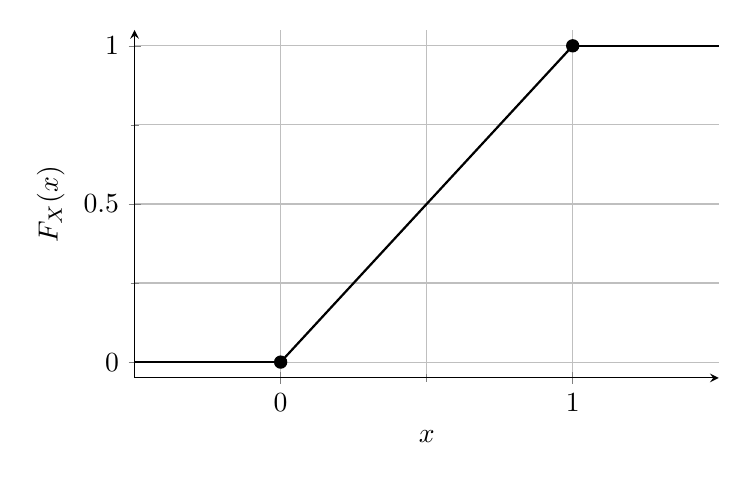
\begin{tikzpicture}
        \begin{axis}[
        width=9cm, height=6cm,
        axis lines=left,
        xmin=-0.5, xmax=1.5, ymin=-0.05, ymax=1.05,
        xlabel={$x$}, ylabel={$F_X(x)$},
        xtick={0,1},
        ytick={0,0.5,1},
        yticklabels={\(0\), \(0{.}5\), \(1\)},
        grid=both, minor tick num=1
        ]
        % Tramo izquierdo: F(x)=0 para x<0
        \addplot[thick, domain=-0.5:0] {0};

        % Tramo lineal: F(x)=x en [0,1]
        \addplot[thick, domain=0:1] {x};

        % Tramo derecho: F(x)=1 para x>1
        \addplot[thick, domain=1:1.5] {1};

        % Puntos extremos (continua, puntos llenos)
        \addplot[only marks, mark=*, mark size=2.2pt]
            coordinates {(0,0) (1,1)};
        \end{axis}
        \end{tikzpicture}
    \end{figure}
\end{example}

Algunas propiedades de las funciones de distribución.

\begin{proposition}
    Si $F_X$ es una función de distribución, entonces valen:
    \begin{itemize}
        \item[\textnormal{(D1)}] $F_X$ es creciente.
        \item[\textnormal{(D2)}] $\lim_{t \to +\infty} F_X(t) = 1$ y $\lim_{t \to -\infty} F_X(t) = 0$
        \item[\textnormal{(D3)}] $F_X$ es continua a derecha. Es decir,
        \begin{equation*}
            \lim_{t \to t_0^+} F_X(t) = F_X(t_0).
        \end{equation*}
    \end{itemize}
\end{proposition}

\begin{proof}
    (D1) Si $a \leq b$, entonces $\{X \leq a\} \subseteq \{X \leq b\}$. Por lo tanto,
    \begin{align*}
        P(X \leq a) &\leq P(X \leq b) \\
        F_X(a) &\leq F_X(b).
    \end{align*}

    \medskip

    (D2) Si $a_n \nearrow + \infty$, entonces 
    \begin{equation*}
        (-\infty, a_n] \subseteq (-\infty, a_{n+1}].
    \end{equation*}
    Consideramos $\R = \bigcup_{n \in \N} (-\infty, a_n]$. Entonces,
    \begin{equation*}
        \lim_{n \to \infty} F_X(a_n) = P_X\left(\bigcup_{n \in \N} (-\infty, a_n]\right) = P_X(\Omega) = 1.
    \end{equation*}
    Para probar límite, simplemente consideramos la secuencia decreciente.

    \medskip

    (D3) Sea $a_n \searrow t_0$. La intersección $\bigcap_{n \in \N} (\infty, a_n] = (-\infty, t_0]$. Entonces,
    \begin{align*}
        \lim_{n \to \infty} F_X(t_n) &= \lim_{n \to \infty} P_X(\infty, a_n] \\
        &=P_X(-\infty, t_0] \\
        &= F_X(t_0).
    \end{align*}
\end{proof}

Es más, no lo vemos, pero las condiciones (D1), (D2) y (D3) suficientes para determinar si $F_X$ es una función de distribución.


\section{Tipos de variables aleatorias}

Primero una definición.

\begin{definition}
    Si $X$ e $Y$ son variables aleatorias con $F_X = F_Y$, entonces decimos que $X$ se distribuye como $Y$. Esto se escribe como $X \sim Y$.
\end{definition}

Clasificamos las variables aleatorias en cuatro grupos:
\begin{enumerate}
    \item \textbf{Discretas.}  
    $X$ es discreta si existe un conjunto numerable $A \subseteq \R$ tal que $P_X(A) = 1$.  
    En este caso, la función de distribución $F_X$ es \emph{escalonada}.

    \item \textbf{Absolutamente continuas.}  
    $X$ es absolutamente continua si existe una función $f_X : \R \to [0,\infty)$, llamada \emph{densidad de probabilidad}, tal que
    \[
        F_X(t) = \int_{-\infty}^{t} f_X(x)\, dx.
    \]
    En este caso, la probabilidad de un intervalo se calcula como
    \[
        P(a \leq X \leq b) = \int_a^b f_X(x)\, dx.
    \]

    \item \textbf{Mixtas.}  
    $X$ es mixta cuando su distribución tiene una parte discreta y una parte absolutamente continua.  
    Es decir, existe una descomposición
    \[
        P_X = \alpha P_d + (1-\alpha) P_c, \qquad 0<\alpha<1,
    \]
    donde $P_d$ es una medida discreta y $P_c$ una medida absolutamente continua.

    \item \textbf{Otras.}  
    Existen distribuciones que no encajan en las categorías anteriores (por ejemplo, distribuciones \emph{singulares} como la de Cantor).  
    En este curso no nos vamos a preocupar por ellas.
\end{enumerate}


\section{Variables aleatorias discretas}

Una definición previa:

\begin{definition}
    Llamamos el \emph{rango} de una variable aleatoria $X$ al conjunto
    \[
        R_X = \{ t \in \R \mid P_X(t) > 0 \}.
    \]
\end{definition}

Veamos distintos tipos de variables aleatorias discretas:

\begin{enumerate}
    \item \textbf{Bernoulli.}  
    Sea $p \in [0,1]$. Una variable $X \sim \mathrm{Bernoulli}(p)$ toma valores en $\{0,1\}$ con
    \[
        P(X=1) = p, \qquad P(X=0) = 1-p.
    \]

    \item \textbf{Binomial.}  
    Sea $n \in \N$ y $p \in [0,1]$. Una variable $X \sim \mathrm{Binomial}(n,p)$ representa la cantidad de éxitos en $n$ ensayos independientes de Bernoulli$(p)$. Su rango es $\{0,1,\ldots,n\}$ y
    \[
        P(X=k) = \binom{n}{k} p^k (1-p)^{\,n-k}, \qquad 0 \leq k \leq n.
    \]

    \item \textbf{Geométrica.}  
    Sea $p \in (0,1]$. Una variable $X \sim \mathrm{Geom}(p)$ modela el número de ensayos hasta obtener el primer éxito. Su rango es $\{1,2,3,\ldots\}$ y
    \[
        P(X=k) = (1-p)^{k-1} p, \qquad k \geq 1.
    \]
\end{enumerate}
